\documentclass[a4paper,12pt]{article}

% Essential packages for mathematical writing and figures
\usepackage{amsmath}    % For math environments like align
\usepackage{amssymb}    % For additional math symbols
\usepackage{amsfonts}   % For mathematical fonts
\usepackage{graphicx}   % For including images
\usepackage{caption}    % For customizing captions
\usepackage{subcaption} % For subfigures
\usepackage{enumitem}
\usepackage{subcaption} % For custom enumerations
\usepackage{hyperref}   % For hyperlinks
\usepackage{geometry}   % For custom page layout
\geometry{a4paper, margin=1in}

% Additional formatting
\numberwithin{equation}{section} % Number equations by section
\setlength{\parindent}{0pt}      % No paragraph indentation
\setlength{\parskip}{1em}        % Add space between paragraphs

\begin{document}

% Title Section
\title{\textbf{Cathode Ray Oscilloscope}}
\author{EE24BTECH11065-Spoorthi\\EE24BTECH11023-Rasagna}
\date{\today}
\maketitle
\begin{itemize}
\item An oscilloscope is an electronic measuring instrument used to display and analyze the waveform of electronic signals.
\item It shows how a signal varies with time, presenting it as a graph where the horizontal axis represents time and the vertical axis represents voltage.
\item Oscilloscopes are commonly used in electronics and engineering to observe signal behavior sine waves, square waves, etc,diagnose problems in circuits,Test and debug electronic devices and measure parameters like frequency, amplitude, and phase.
\end{itemize}
The key components of oscilloscope are:
\begin{itemize}
\item Cathode Ray Tube (CRT)
\item Vertical Deflection System
\item Horizontal Deflection System
\item Time Base Generator
\item Trigger Circuit
\item Power Supply
\item Amplifiers (Vertical and Horizontal)
\item Input Section
\item Graticule (Screen)
\item Control Panel
\end{itemize}
\section*{Generating Lissajous Figures}
\textbf{Components required for this experiment}
\begin{itemize}
    \item Cathode Ray Oscilloscope
    \item Function Generator
    \item BNC cables or BNC connectors
\end{itemize}
Lissajous figures are complex patterns resulting from the interaction of two harmonic motions, typically visualized on an oscilloscope or generated using mathematical modeling.
\section{Figure 1}
The inputs taken for the two signals are given in Figure 1:
\begin{figure}[h!]
    \centering
    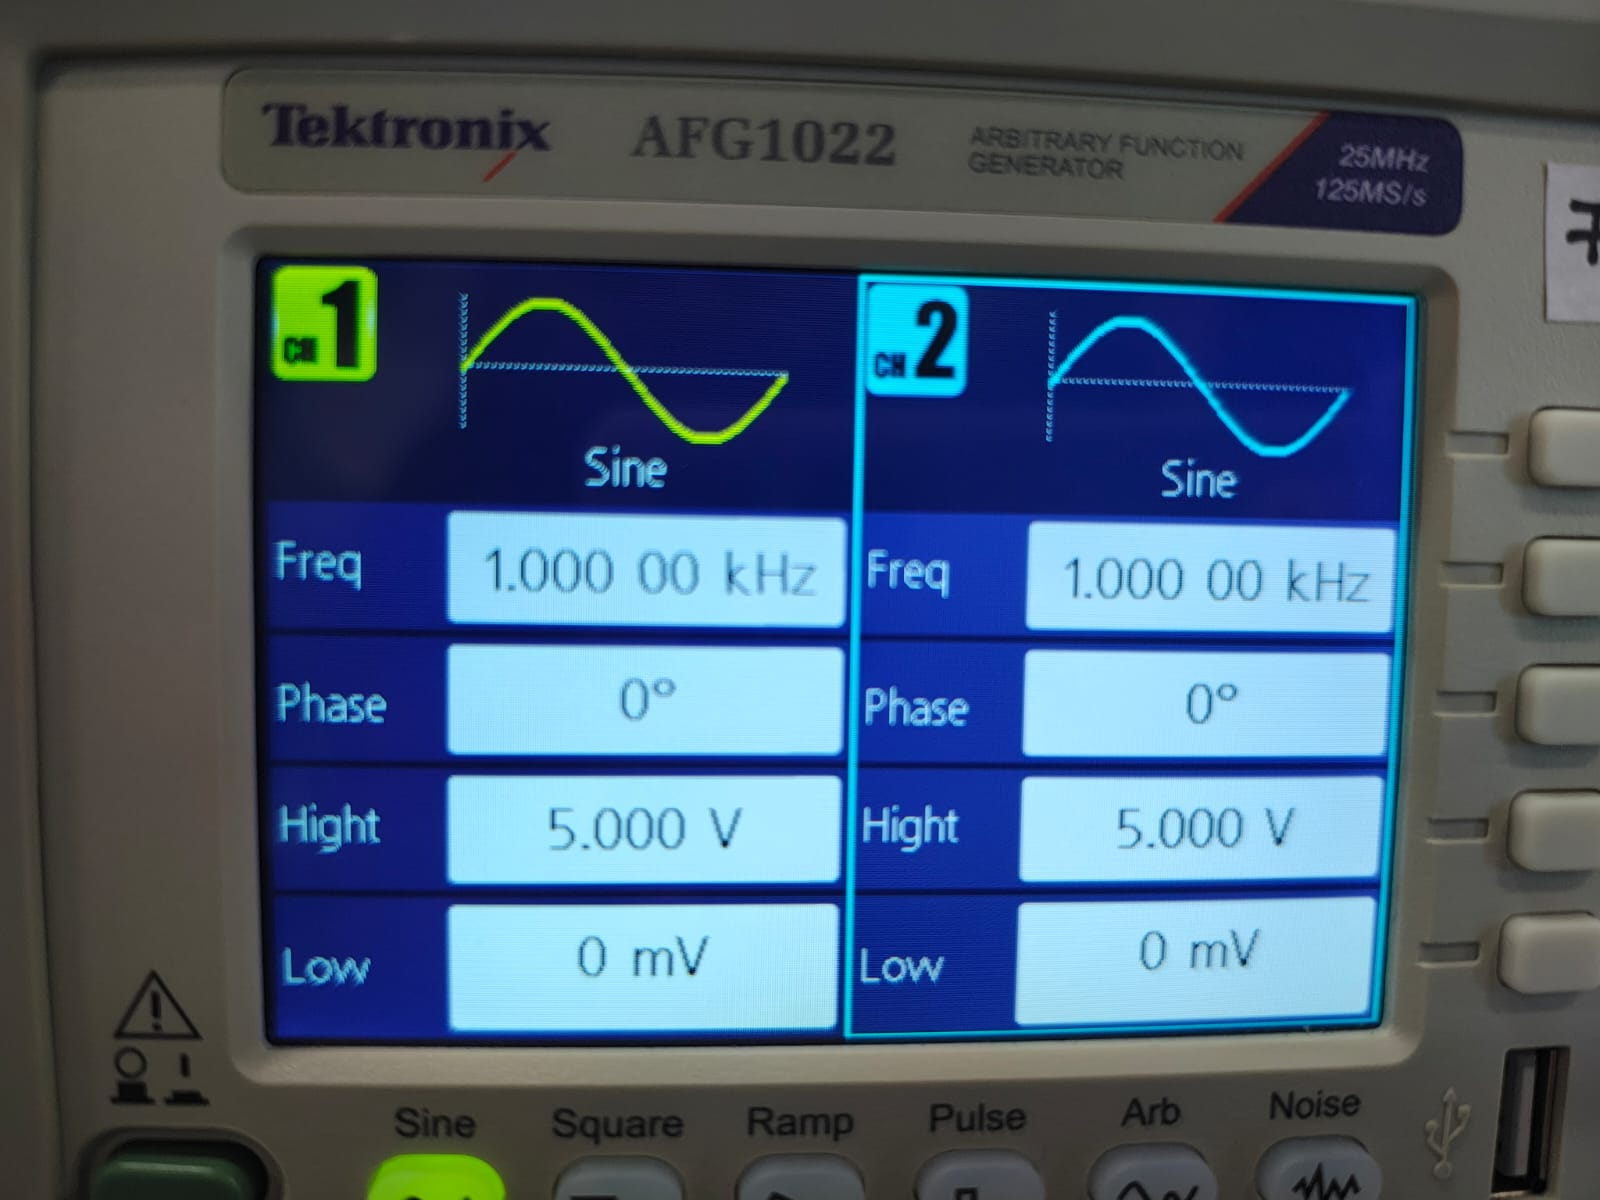
\includegraphics[width=0.5\linewidth]{Tables/Table1.jpeg} 
    \caption{}
\end{figure}
\begin{align}
    x(t) &= A \sin \omega t \\
    y(t) &= A \sin \omega t 
\end{align}
In our case,
\begin{align}
    A &= 5 \, \text{V (peak)}, \\
    f &= 1 \times 10^3 \, \text{Hz}, \\
    \omega &= 2 \pi f = 2 \pi (10^3) \, \text{rad/s} = 2 \times 10^3 \, \text{rad/s}.
\end{align}
On subtracting equations (1) and (2), we get:
\begin{align}
    x(t) - y(t) &= 0, \\
    y(t) &= x(t).
\end{align}
On plotting $y(t)$ vs $x(t)$, we get a $y = x$ straight line.\\
\begin{figure}[htbp]
    \centering
    \begin{minipage}{0.45\textwidth}
        \centering
        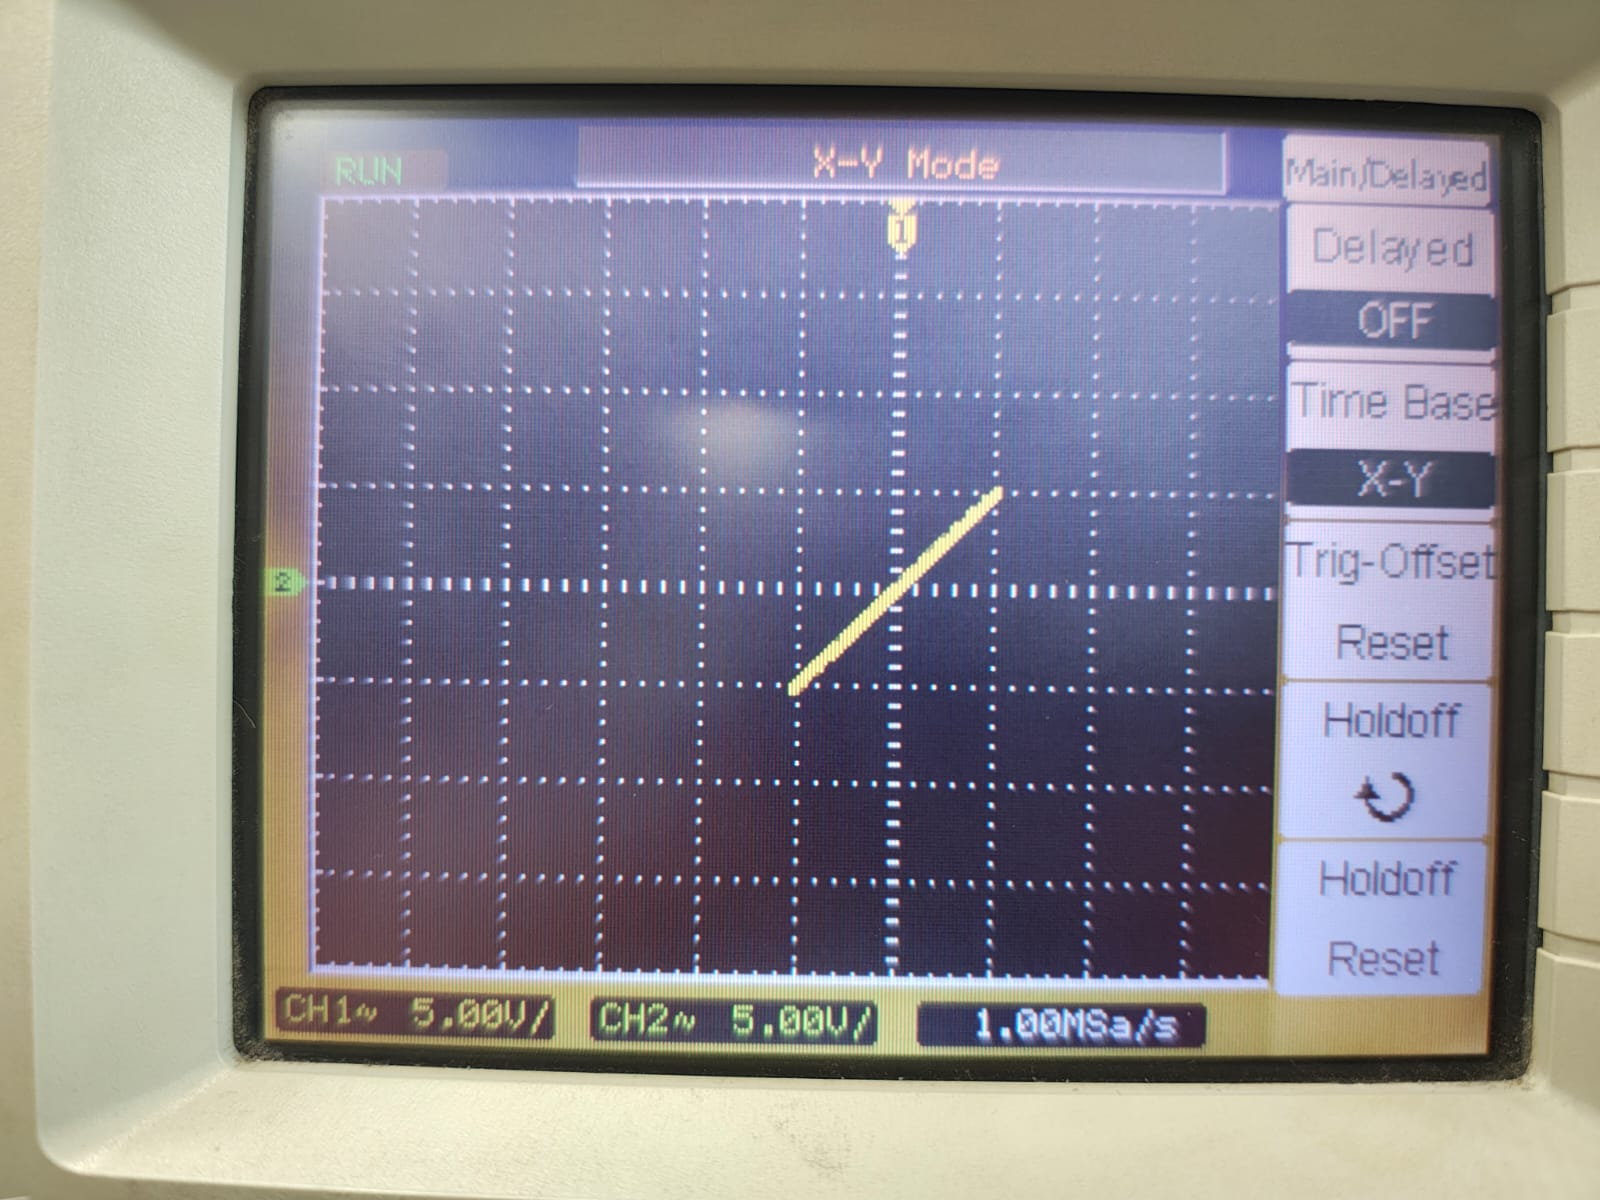
\includegraphics[width=\linewidth]{Graphs/Graph1.jpeg}
        \caption{Obtained}
    \end{minipage}
    \hfill
    \begin{minipage}{0.45\textwidth}
        \centering
        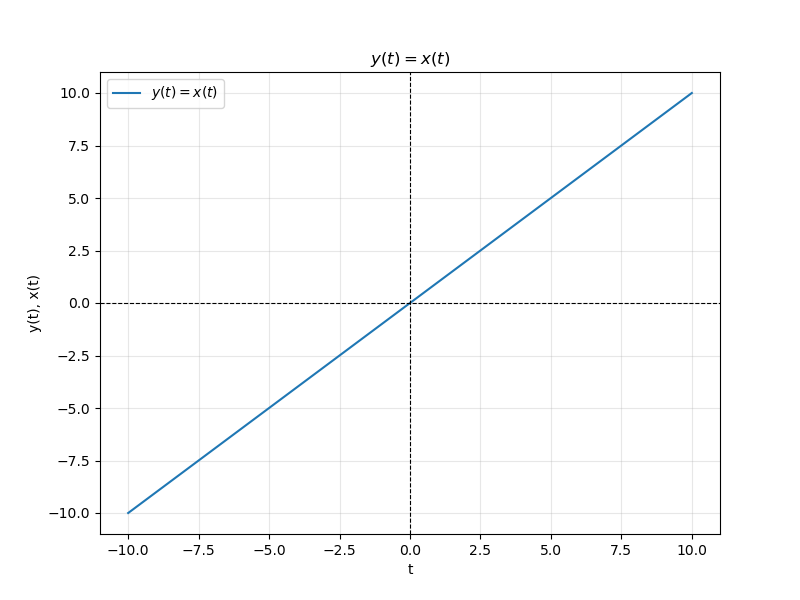
\includegraphics[width=\linewidth]{Python plots/lab3.png} 
        \caption{Generated}
    \end{minipage}
\end{figure}
\newpage
\section{Figure 2}
The inputs taken for the two signals are given in Figure 4:
\begin{figure}[h!]
    \centering
    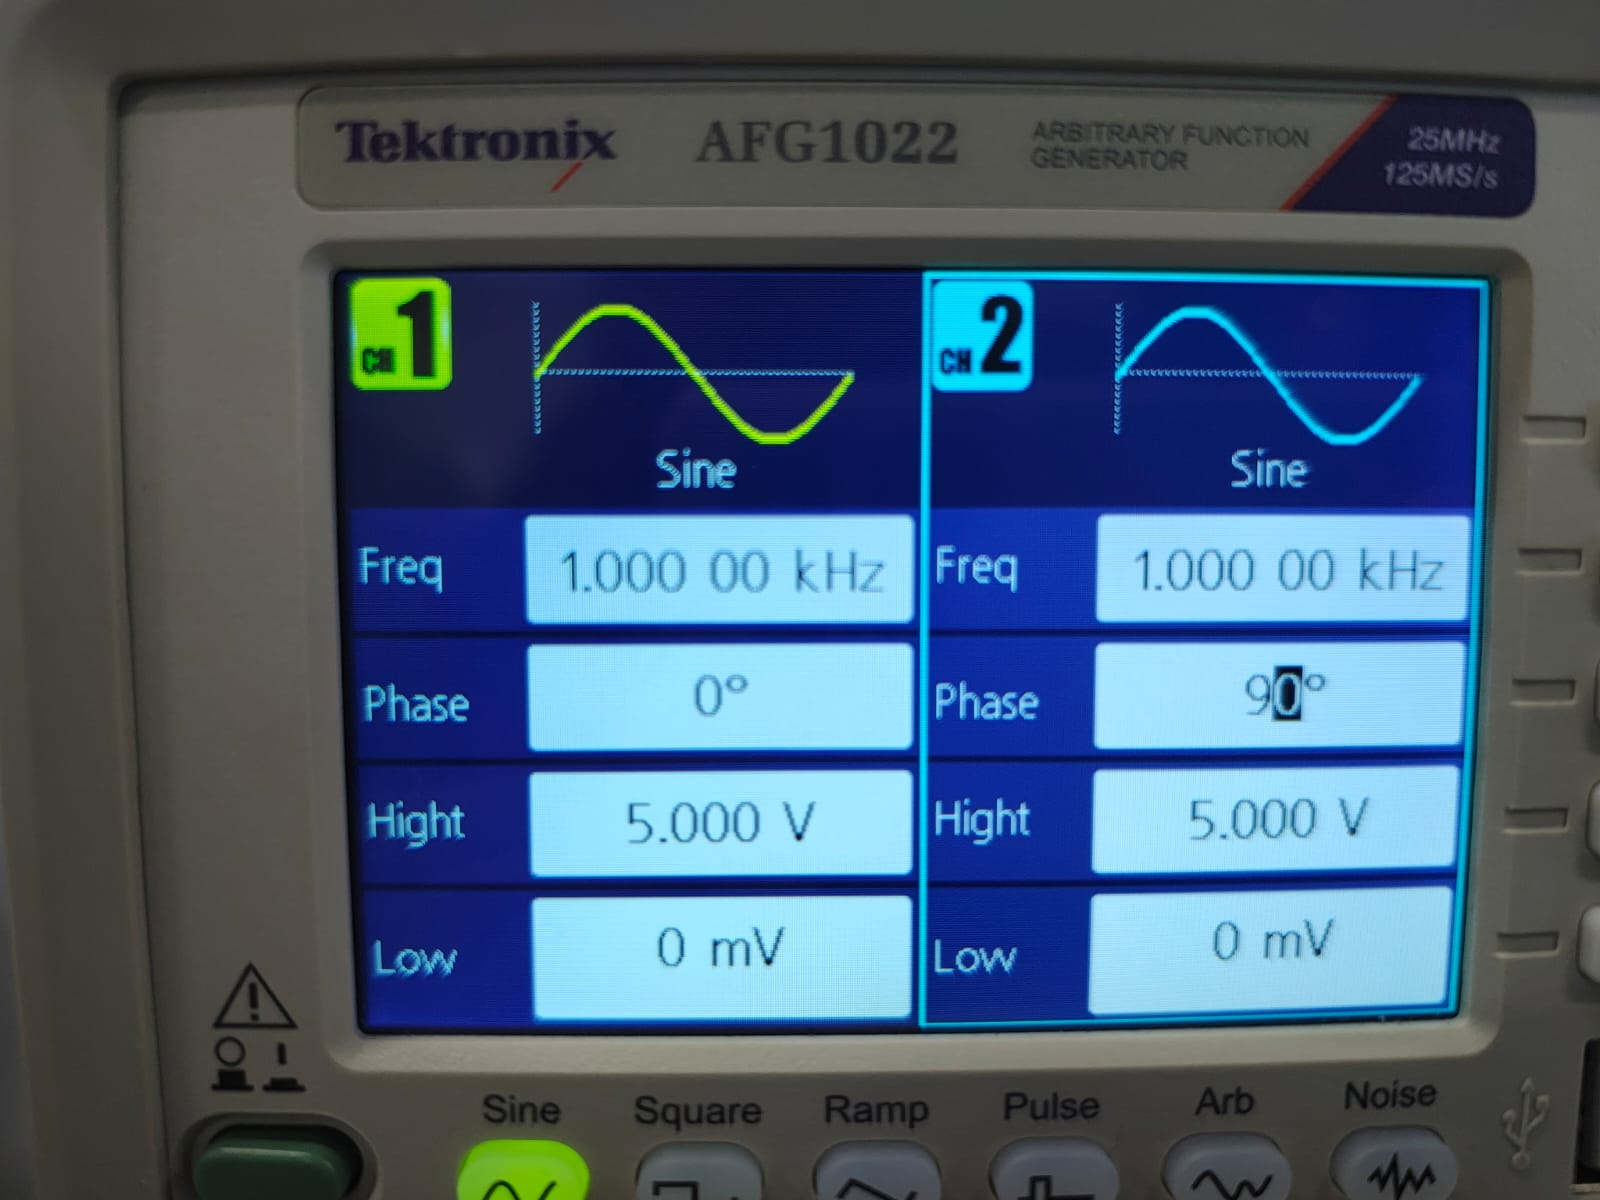
\includegraphics[width=0.5\linewidth]{Tables/Table2.jpeg} 
    \caption{}
\end{figure}\\
\noindent Given:
\begin{align}
    x(t) &= A \sin (\omega t+\frac{\pi}{2}), \\
    y(t) &= A \sin \omega t.
\end{align}
Squaring and adding, we get:
\begin{align}
    x^2(t) + y^2(t) &= A^2 \sin^2 (\omega t +\frac{\pi}{2})+ A^2 \sin^2 \omega t, \\
    x^2 + y^2 &= A^2.
\end{align}
This represents a circle centered at the origin with radius $A=5$.
\begin{figure}[htbp]
    \centering
    \begin{minipage}{0.45\textwidth}
        \centering
        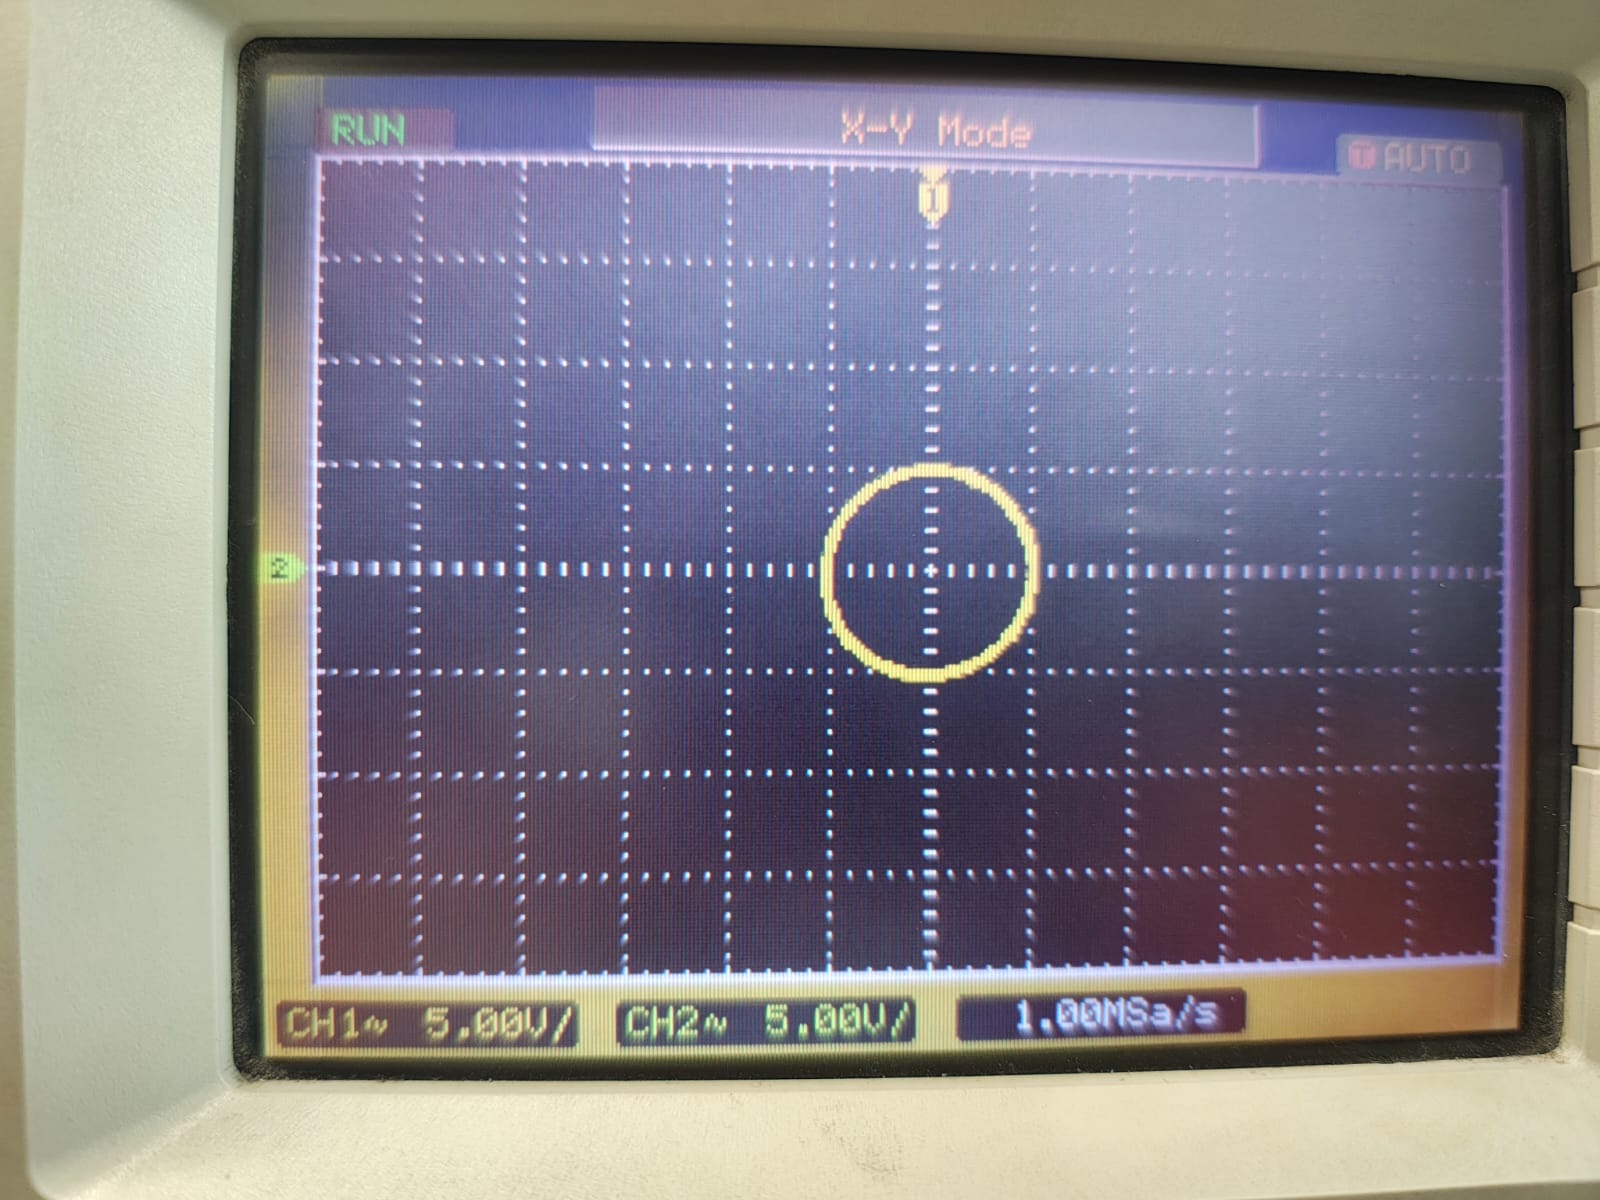
\includegraphics[width=\linewidth]{Graphs/Graph2.jpeg}
        \caption{Obtained}
    \end{minipage}
    \hfill
    \begin{minipage}{0.45\textwidth}
        \centering
        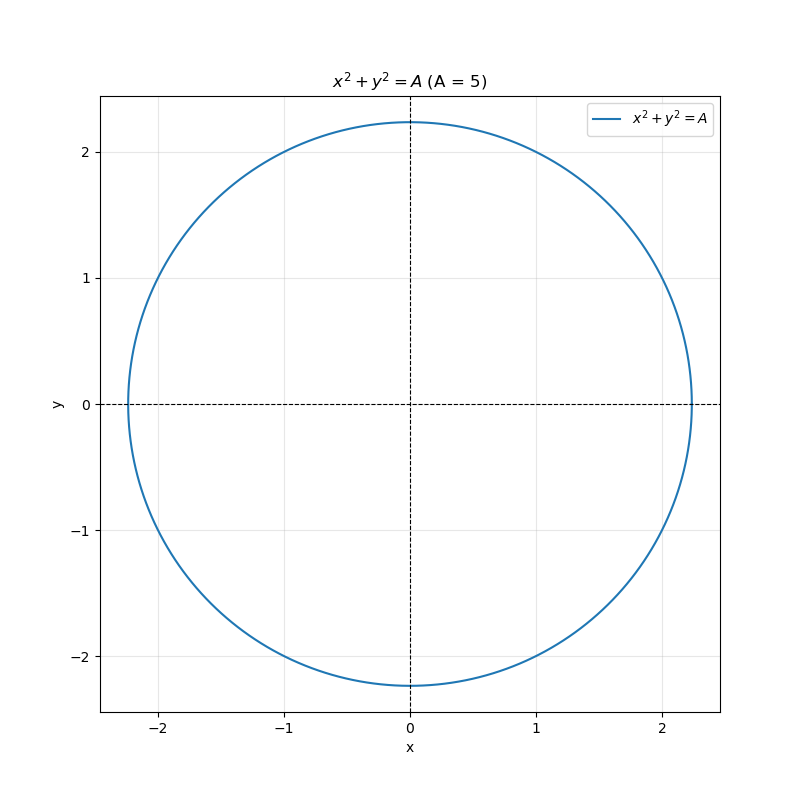
\includegraphics[width=\linewidth]{Python plots/lab4.png} 
        \caption{Generated}
    \end{minipage}
\end{figure}
\newpage
\section{Figure 3}
The inputs taken for the two signals are given in Figure 7:
\begin{figure}[h!]
    \centering
    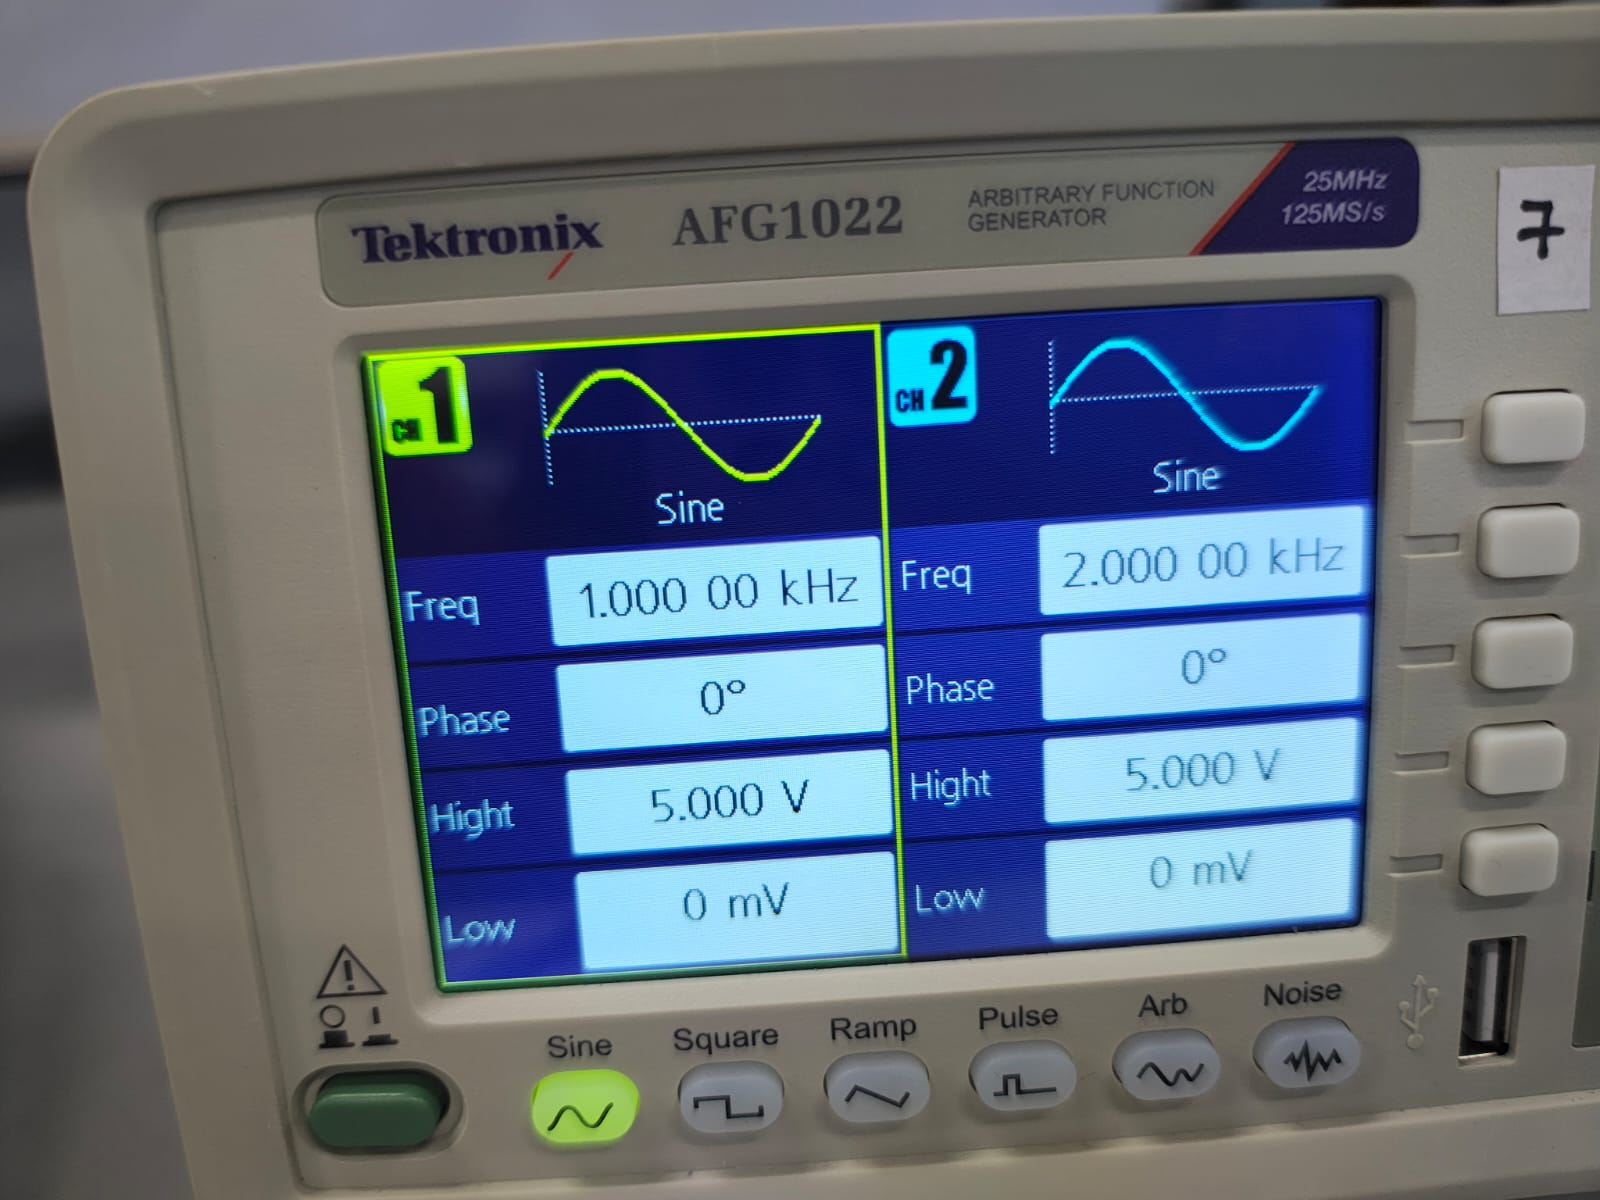
\includegraphics[width=0.5\linewidth]{Tables/Table5.jpeg} 
    \caption{}
\end{figure}\\
\noindent Given:
\begin{align}
    x(t) &= A \sin \omega t, \\
    y(t) &= A \sin(2\omega t).
\end{align}
\begin{align}
    y&=2A{sin(\omega t})\sqrt{1-sin^2{\omega t}}\\
    y&=2x\sqrt{1-\frac{x^2}{A^2}}\\
    \frac{y^2}{4x^2}&=1-\frac{x^2}{A^2}\\
    \frac{x^2}{A^2}+\frac{y^2}{4x^2}&=1\\
    y^2&=4x^2-\frac{4x^4}{A^2}
\end{align}
The graph of the obtained equation is shown below.
\begin{figure}[htbp]
    \centering
    \begin{minipage}{0.45\textwidth}
        \centering
        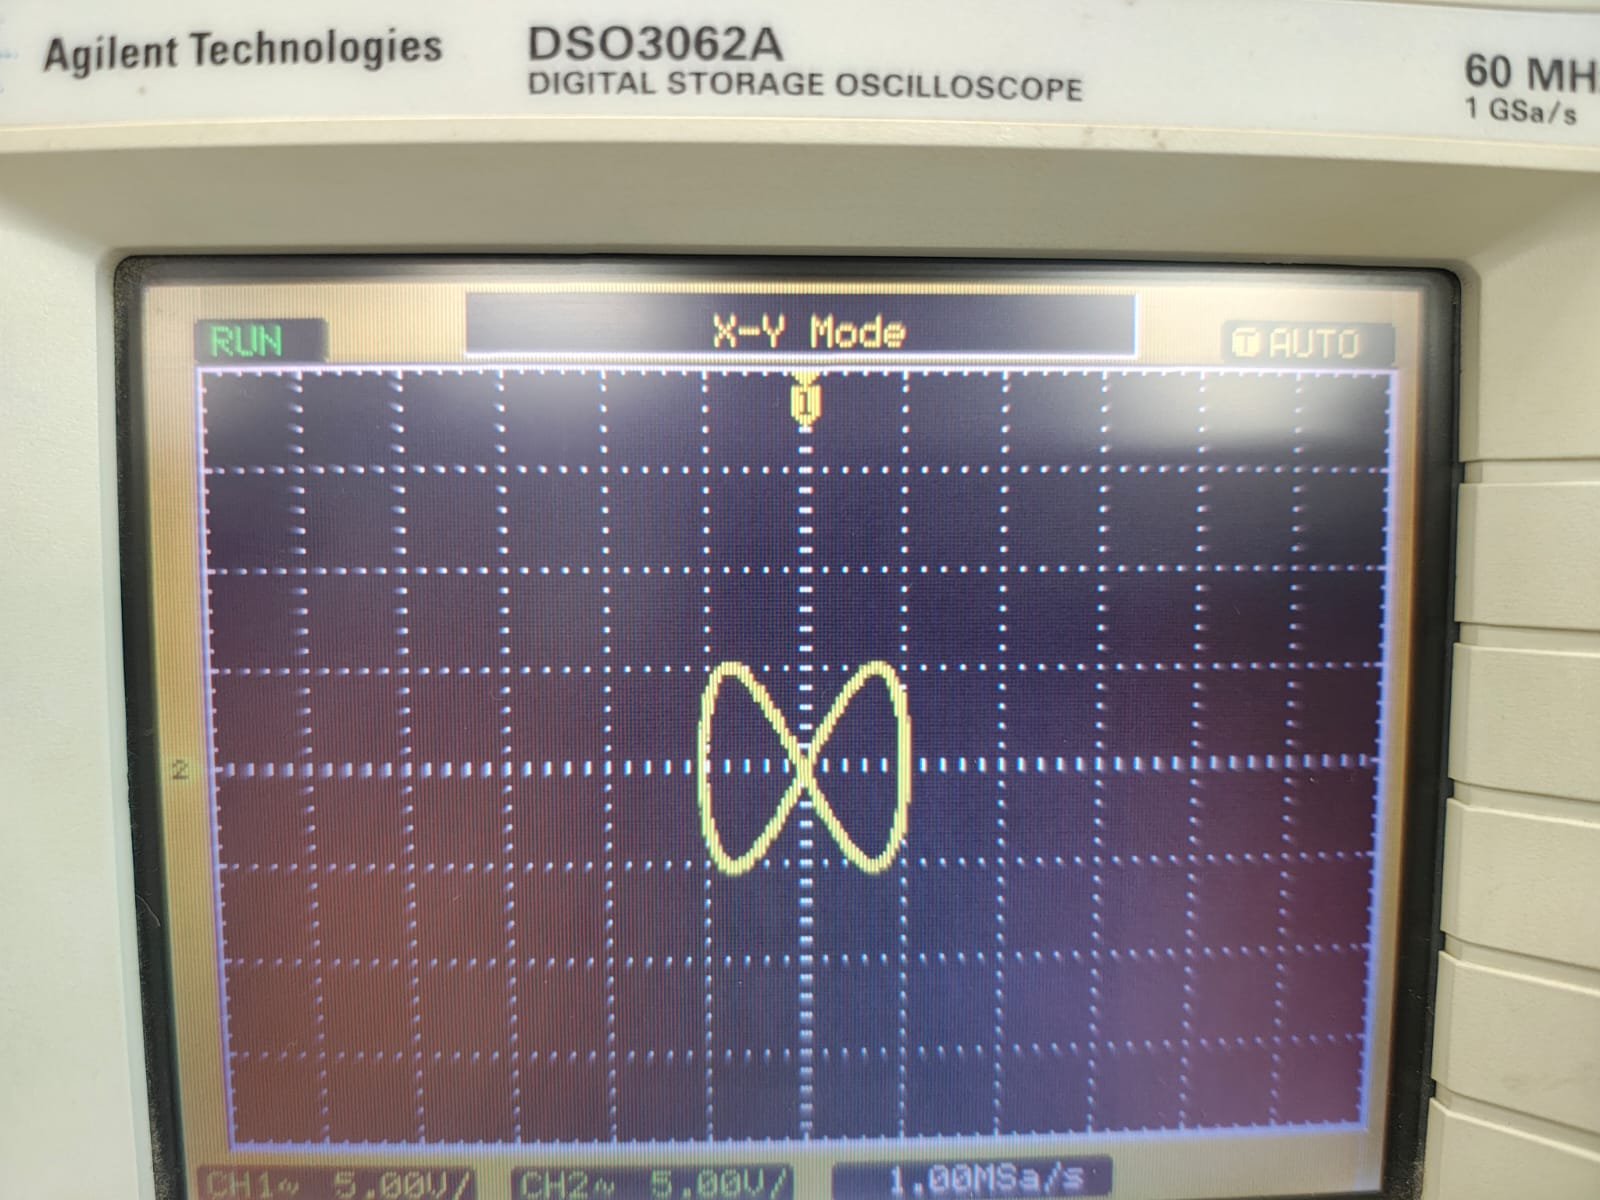
\includegraphics[width=\linewidth]{Graphs/Graph5.jpeg}
        \caption{Obtained}
    \end{minipage}
    \hfill
    \begin{minipage}{0.45\textwidth}
        \centering
        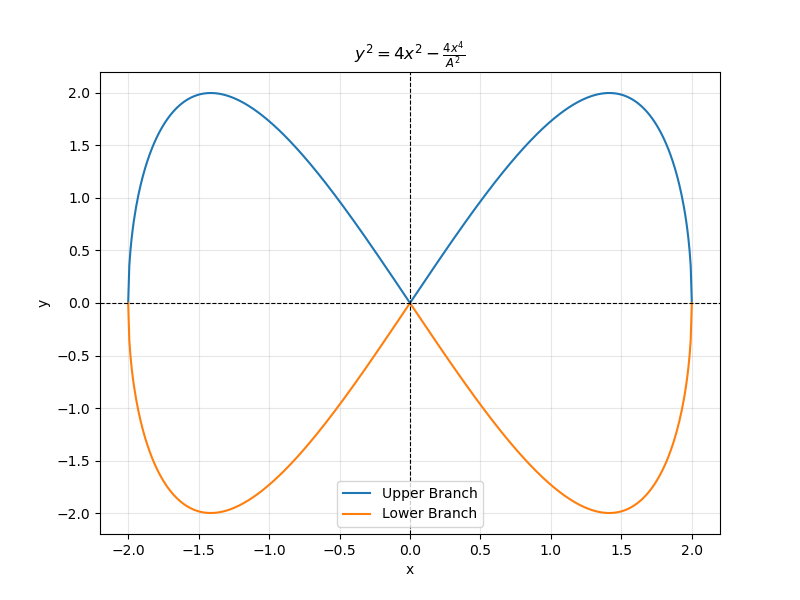
\includegraphics[width=\linewidth]{Python plots/lab1.png} 
        \caption{Generated}
    \end{minipage}
\end{figure}
\newpage
\section{Figure 4}
The inputs taken for the two signals are given in Figure 10:
\begin{figure}[h!]
    \centering
    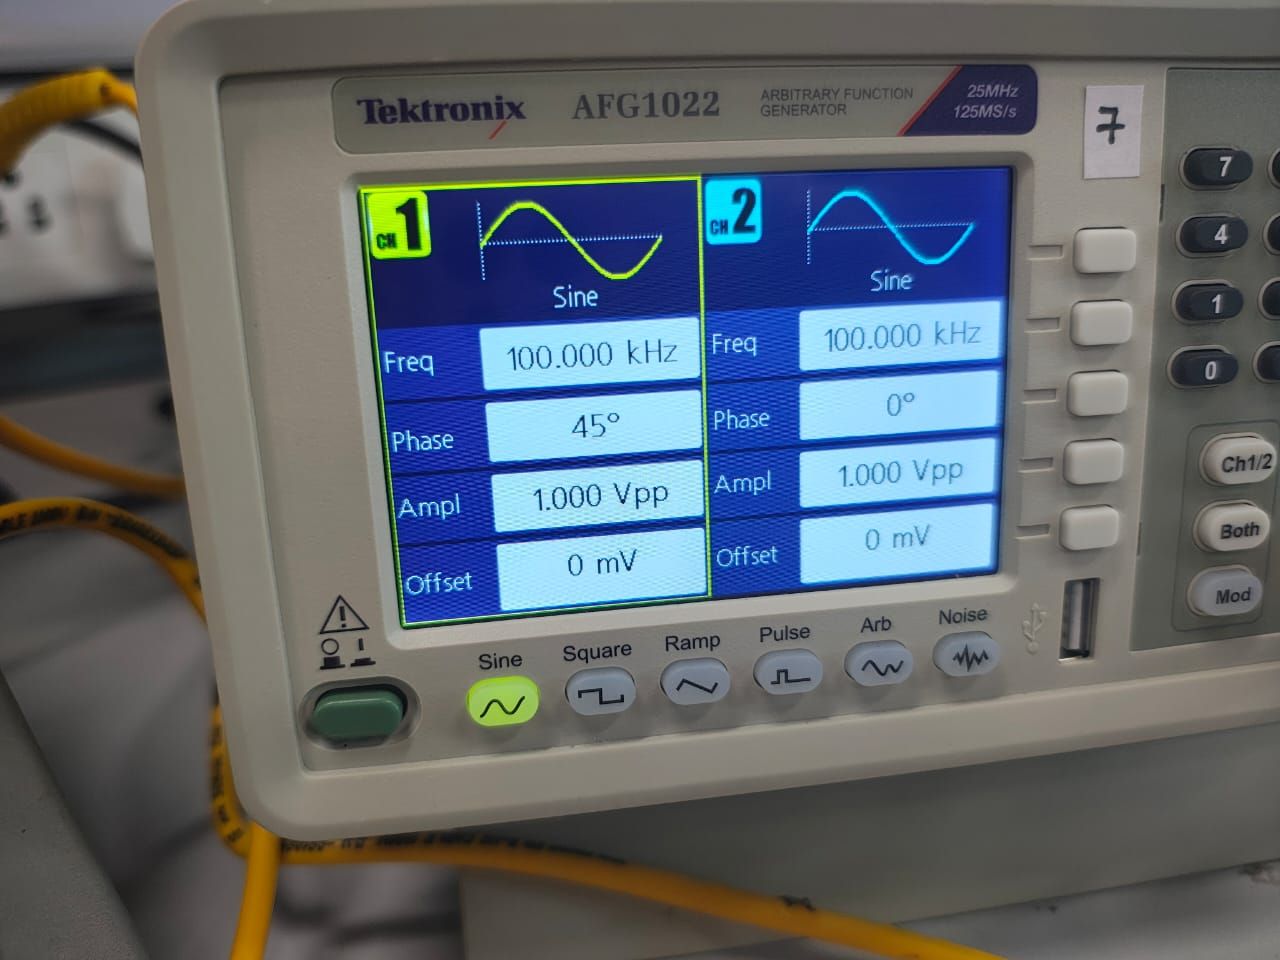
\includegraphics[width=0.5\linewidth]{Tables/Table7.jpeg} 
    \caption{}
\end{figure}\\
\noindent Given:
\begin{align}
    x(t) &= A \sin (\omega t), \\
    y(t) &= A \sin (\omega t+\frac{\pi}{4}).
\end{align}
\begin{align}
    y&=A \bigg(\frac{sin{\omega t}}{\sqrt{2}}+\frac{cos{\omega t}}{\sqrt{2}}\bigg)\\
    y&=\frac{x}{\sqrt{2}}+\frac{A{\sqrt{1-\frac{x^2}{A^2}}}}{\sqrt{2}}\\
    \sqrt{2}y-x & =\sqrt{A^2-x^2}
\end{align}
Squaring on both sides;
\begin{align}
    2x^2+2y^2-2\sqrt{2}xy&=A^2-x^2\\
    A=1Vpp\\
    x^2+y^2-\sqrt{2}xy&=\frac{A^2}{2}
\end{align}
It is the equation of ellipse.
\begin{figure}[htbp]
    \centering
    \begin{minipage}{0.45\textwidth}
        \centering
        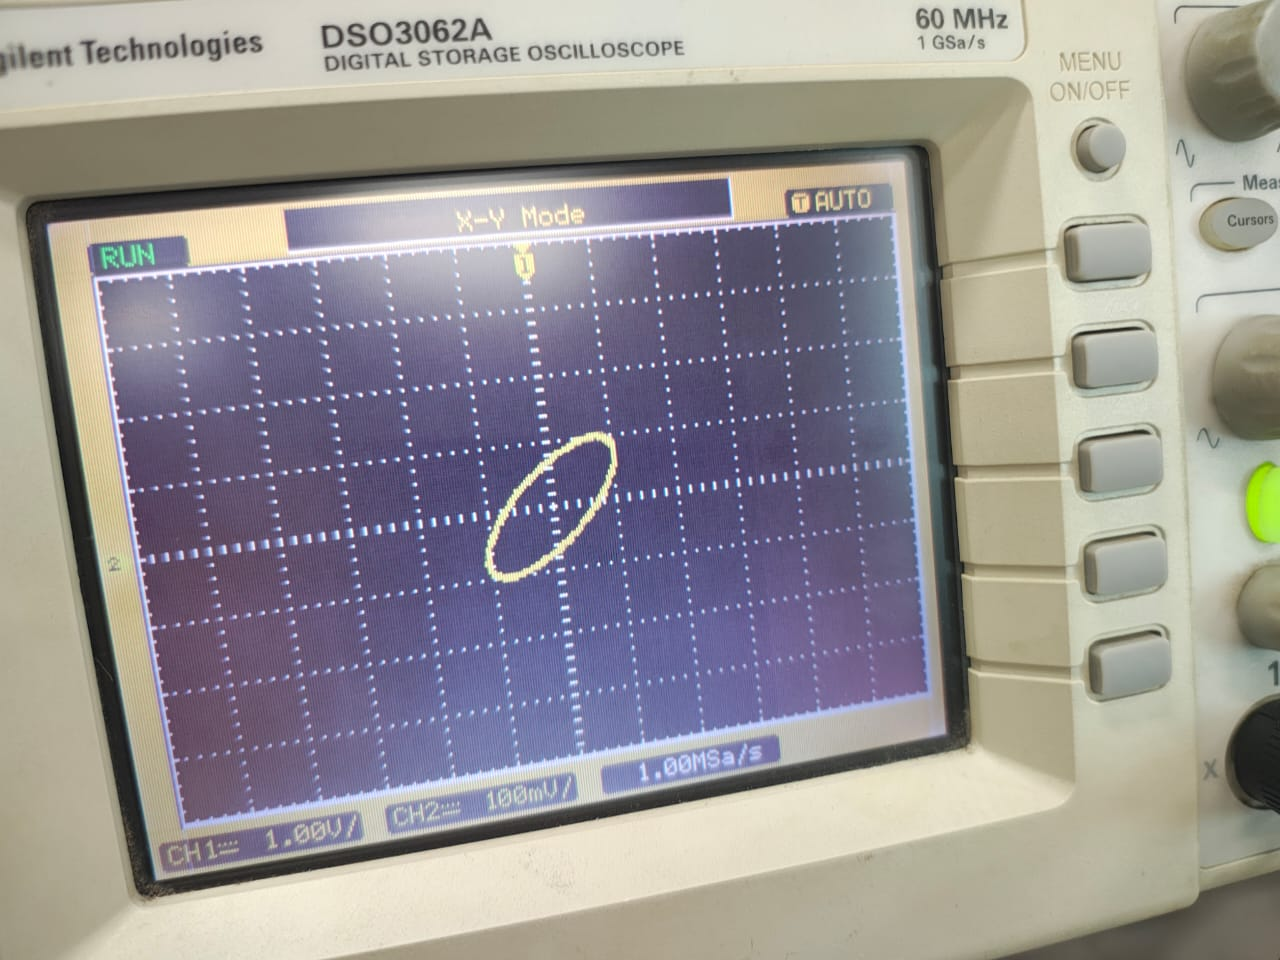
\includegraphics[width=\linewidth]{Graphs/Graph7.jpeg}
        \caption{Obtained}
    \end{minipage}
    \hfill
    \begin{minipage}{0.45\textwidth}
        \centering
        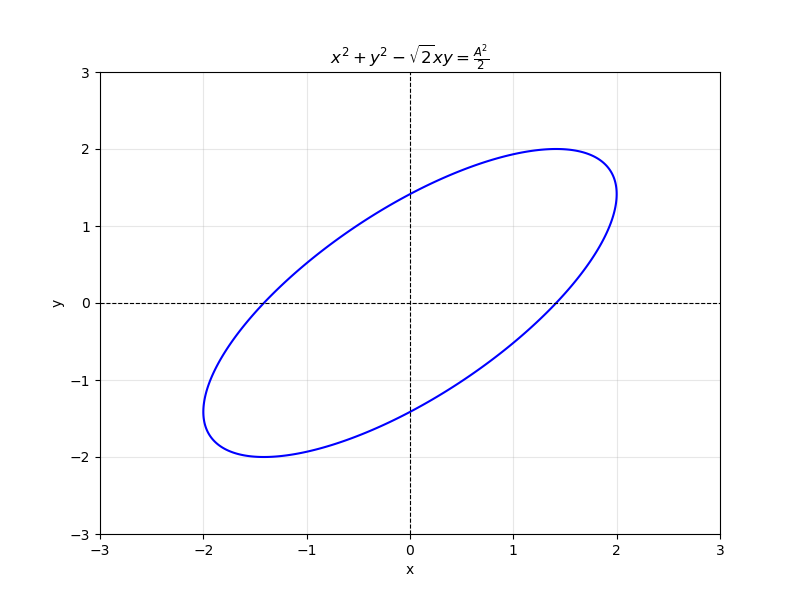
\includegraphics[width=\linewidth]{Python plots/lab2.png} 
        \caption{Generated}
    \end{minipage}
\end{figure}
\newpage
\section{Figure 5}
The inputs taken for the two signals are given in Figure 13:
\begin{figure}[h!]
    \centering
    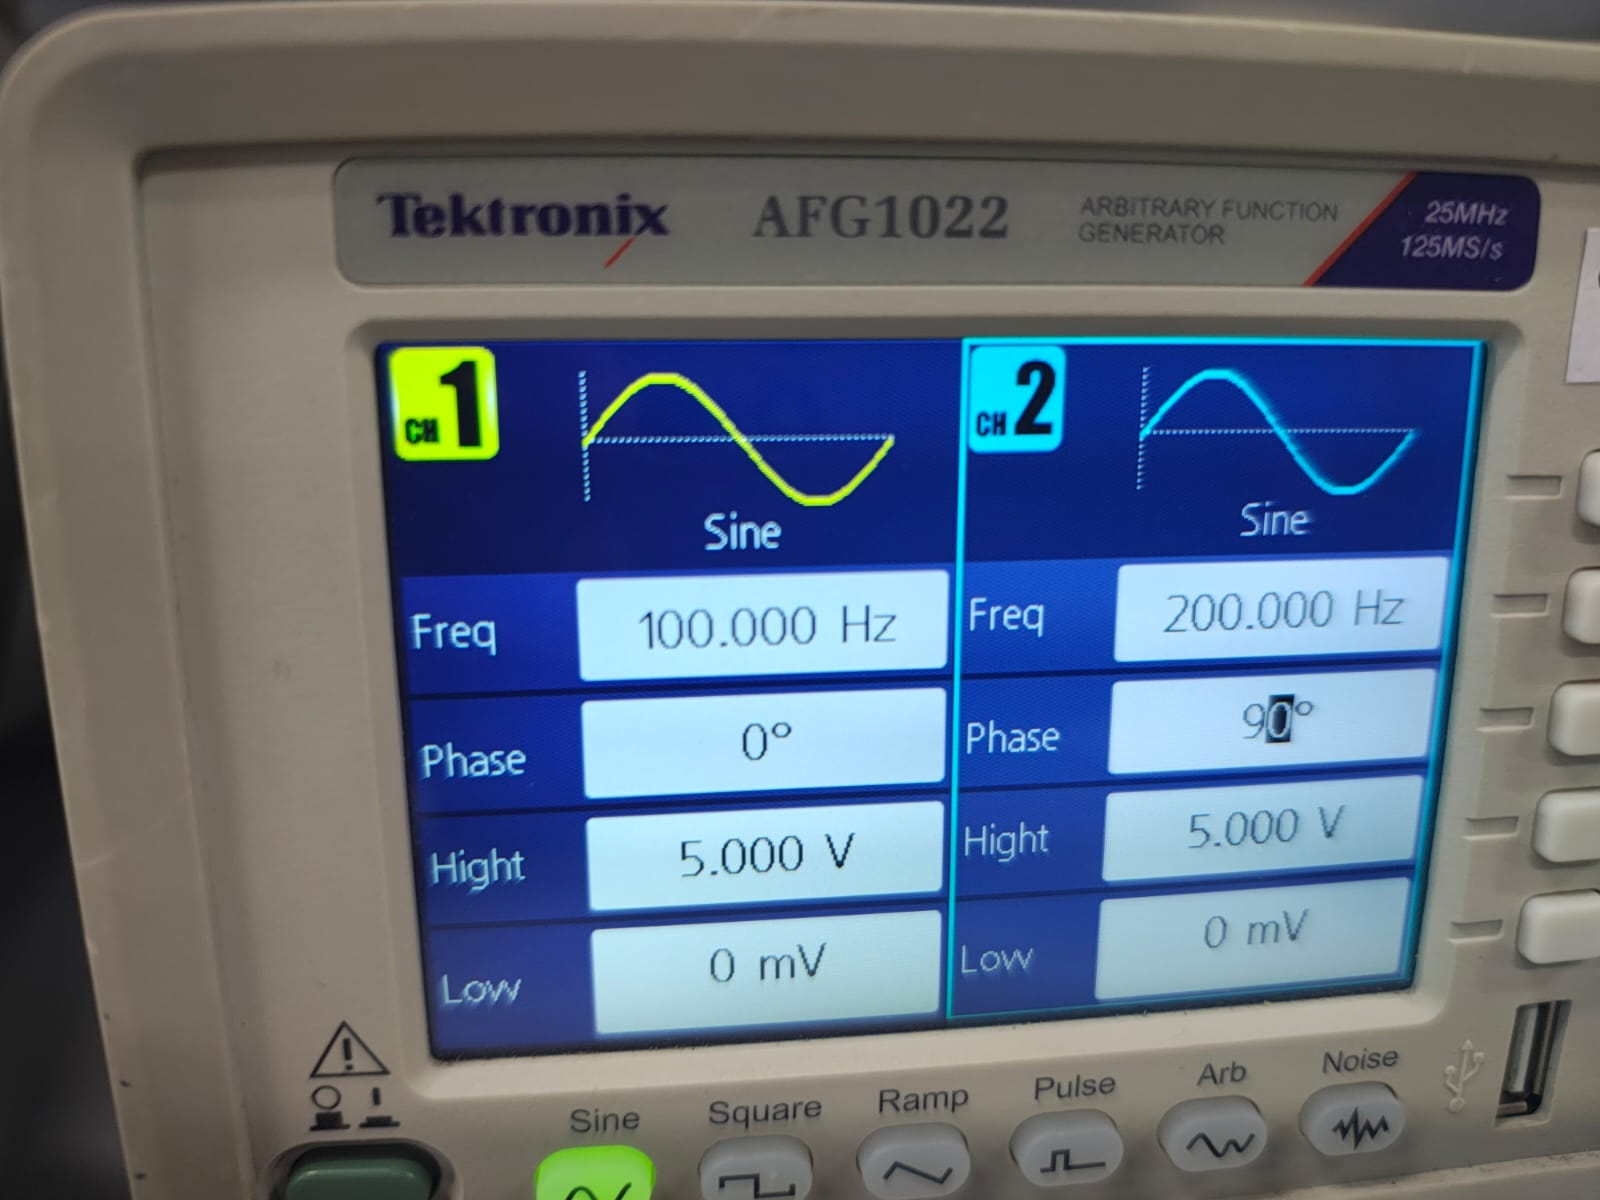
\includegraphics[width=0.5\linewidth]{Tables/Table3.jpeg} 
    \caption{}
\end{figure}
\begin{align}
    x(t) &= A \sin (\omega t), \\
    y(t) &= A \sin (2\omega t+\frac{\pi}{2}).
\end{align}
\begin{align}
    y&=Acos{2 \omega t}\\
    y&=A \bigg(\frac{1-sin^2{\omega t}}{2}\bigg)\\
    y&=\frac{A}{2}-\frac{A}{2}\bigg(\frac{x}{A}\bigg)^2\\
    y&=\frac{A}{2}\bigg(1-\frac{x^2}{A^2}\bigg)
\end{align}
The graph obtained is a parabola as shown;
\begin{figure}[htbp]
    \centering
    \begin{minipage}{0.45\textwidth}
        \centering
        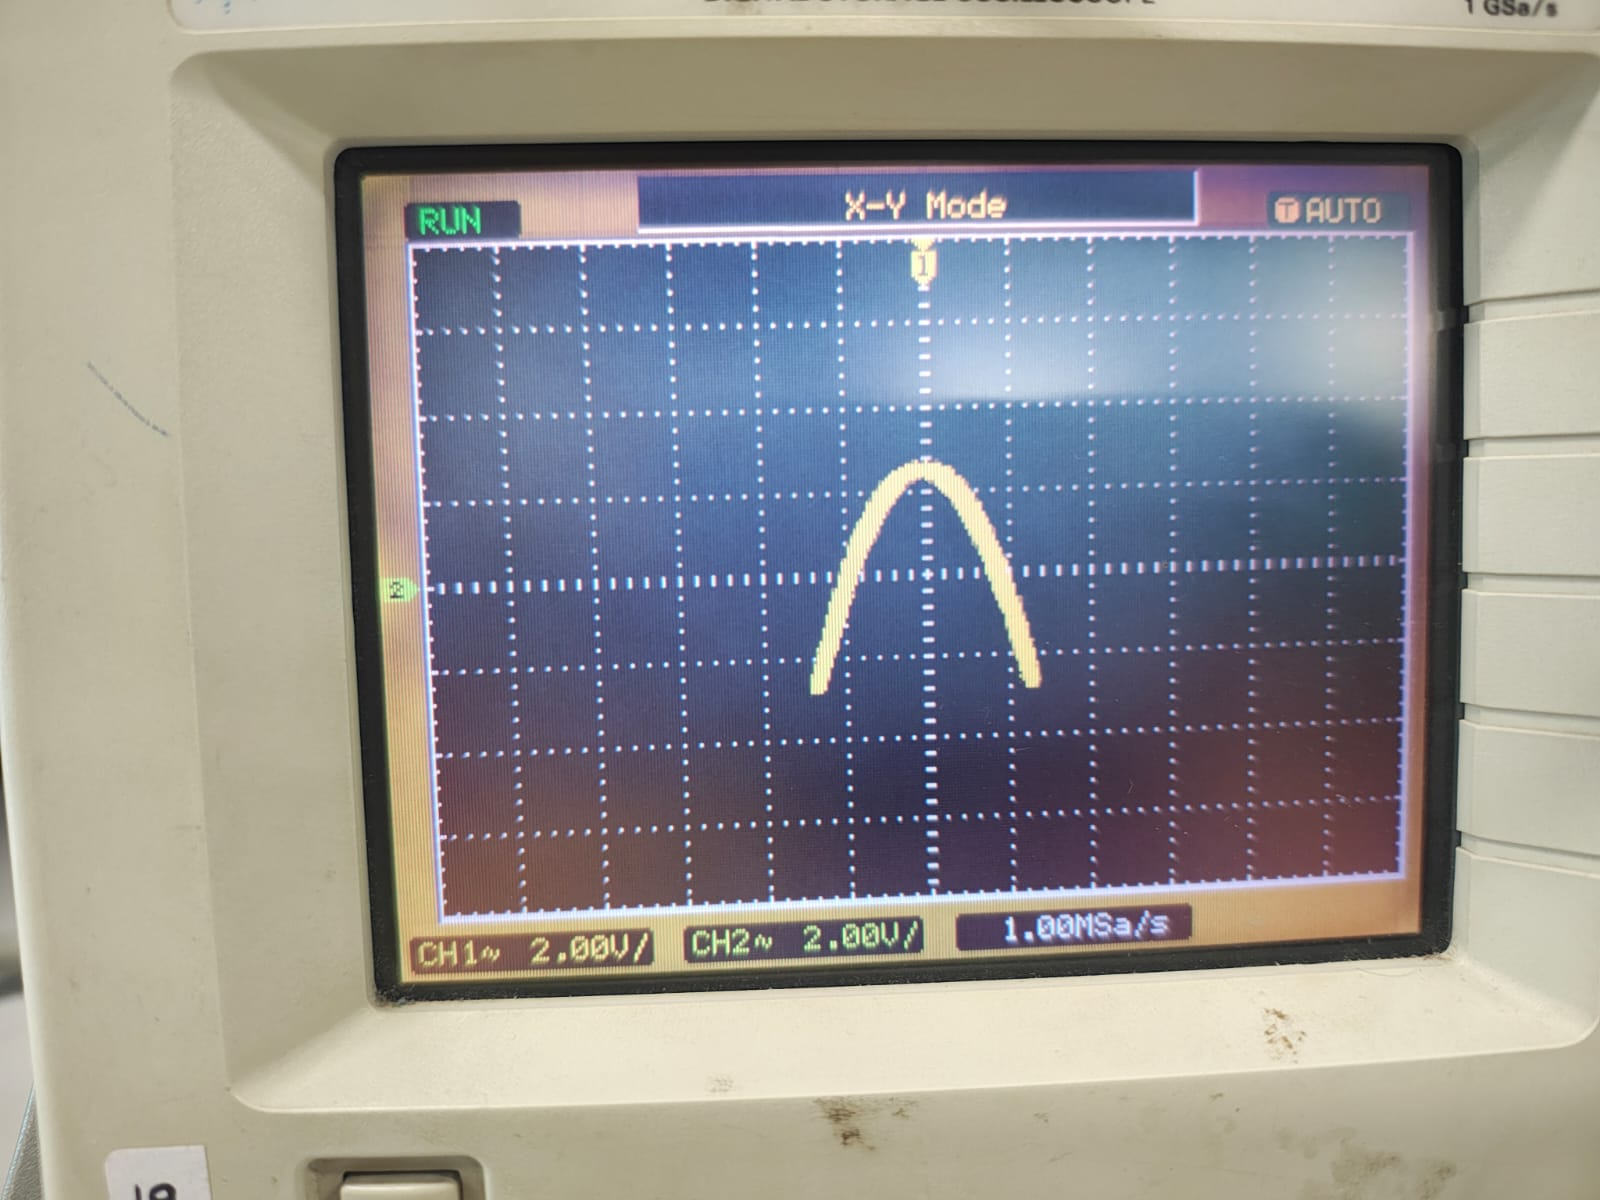
\includegraphics[width=\linewidth]{Graphs/Graph3.jpeg}
        \caption{Obtained}
    \end{minipage}
    \hfill
    \begin{minipage}{0.45\textwidth}
        \centering
        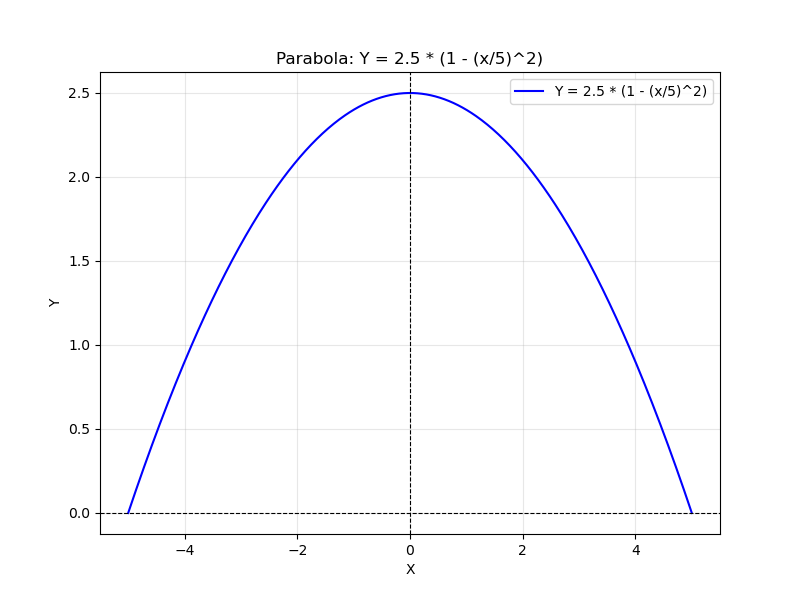
\includegraphics[width=\linewidth]{Python plots/lab5.png} 
        \caption{Generated}
    \end{minipage}
\end{figure}\\
\newpage
\section{Figure 6}
The inputs taken for the two signals are given in Figure 16:
\begin{figure}[h!]
    \centering
    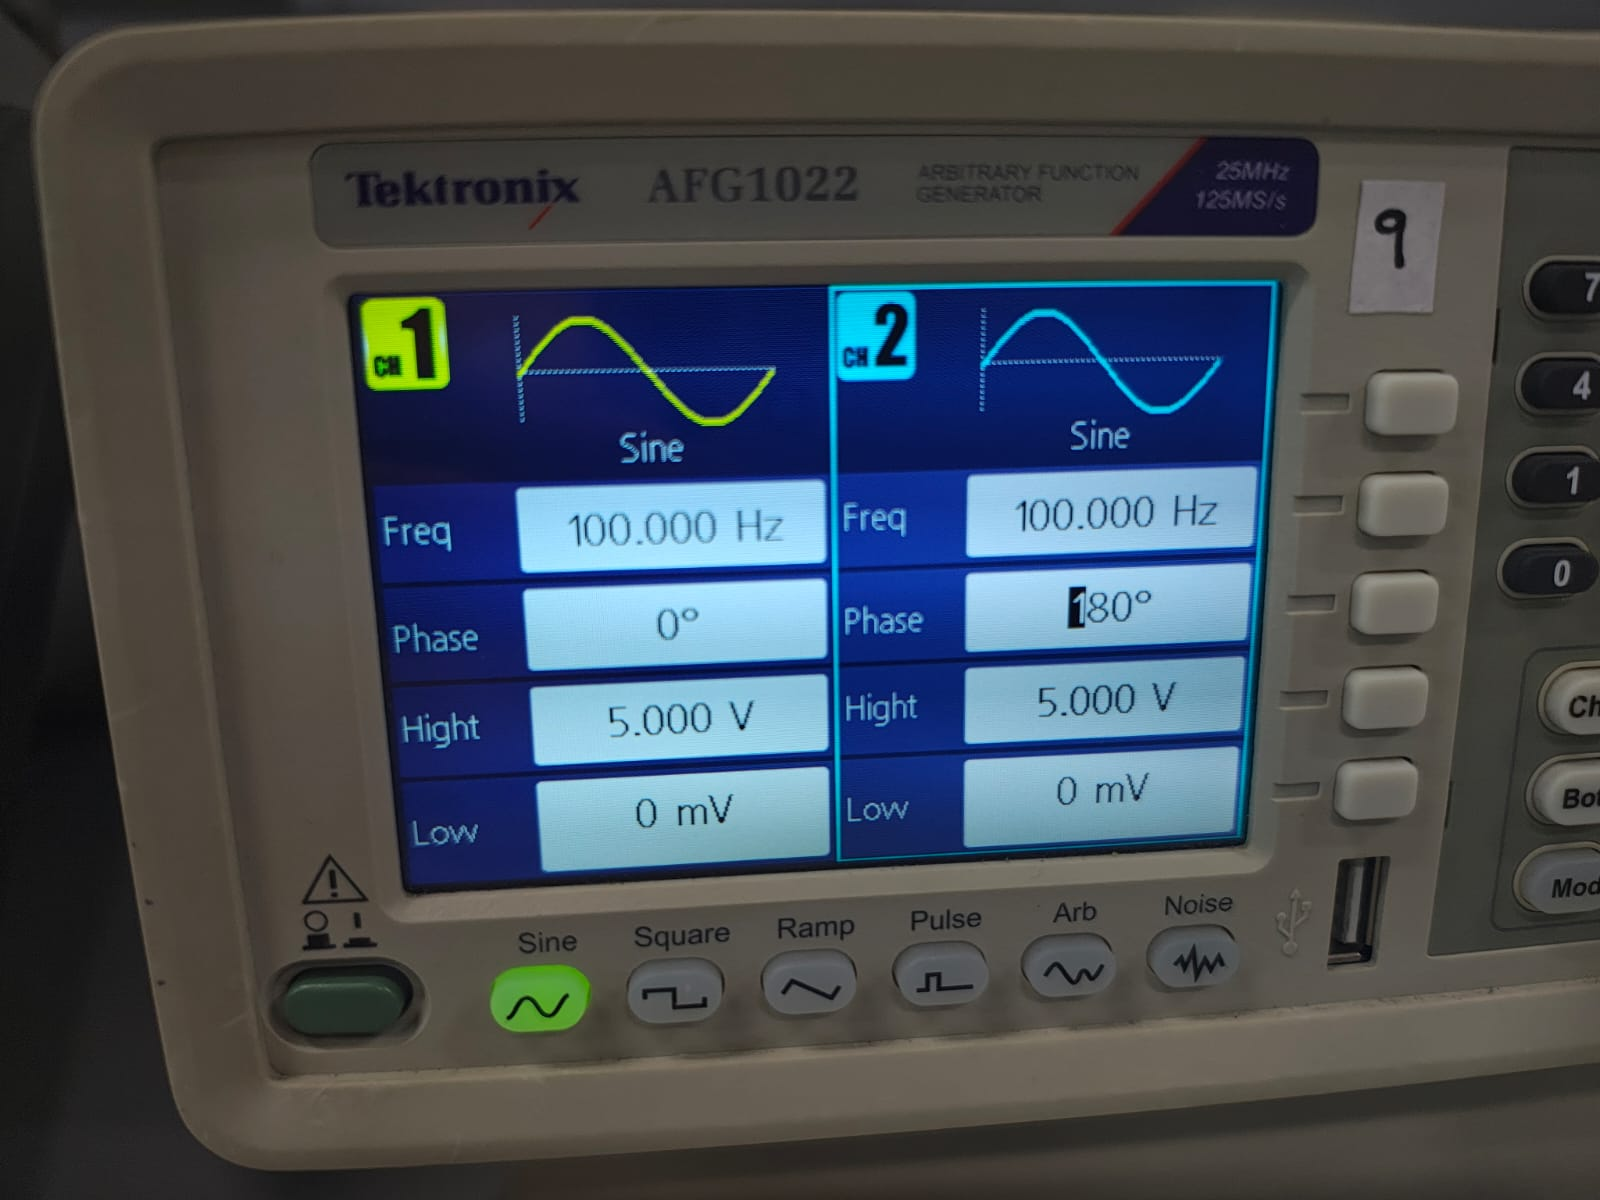
\includegraphics[width=0.5\linewidth]{Tables/Table4.jpeg} 
    \caption{}
\end{figure}
\begin{align}
    x&=Asin{\omega t}\\
    y&=Asin{(\omega t+\pi)}
\end{align}
\begin{align}
    \therefore y&=-Asin{\omega t}\\
    y&=-x
\end{align}
It is the equation of a straight line with slope $-1$.
\begin{figure}[htbp]
    \centering
    \begin{minipage}{0.45\textwidth}
        \centering
        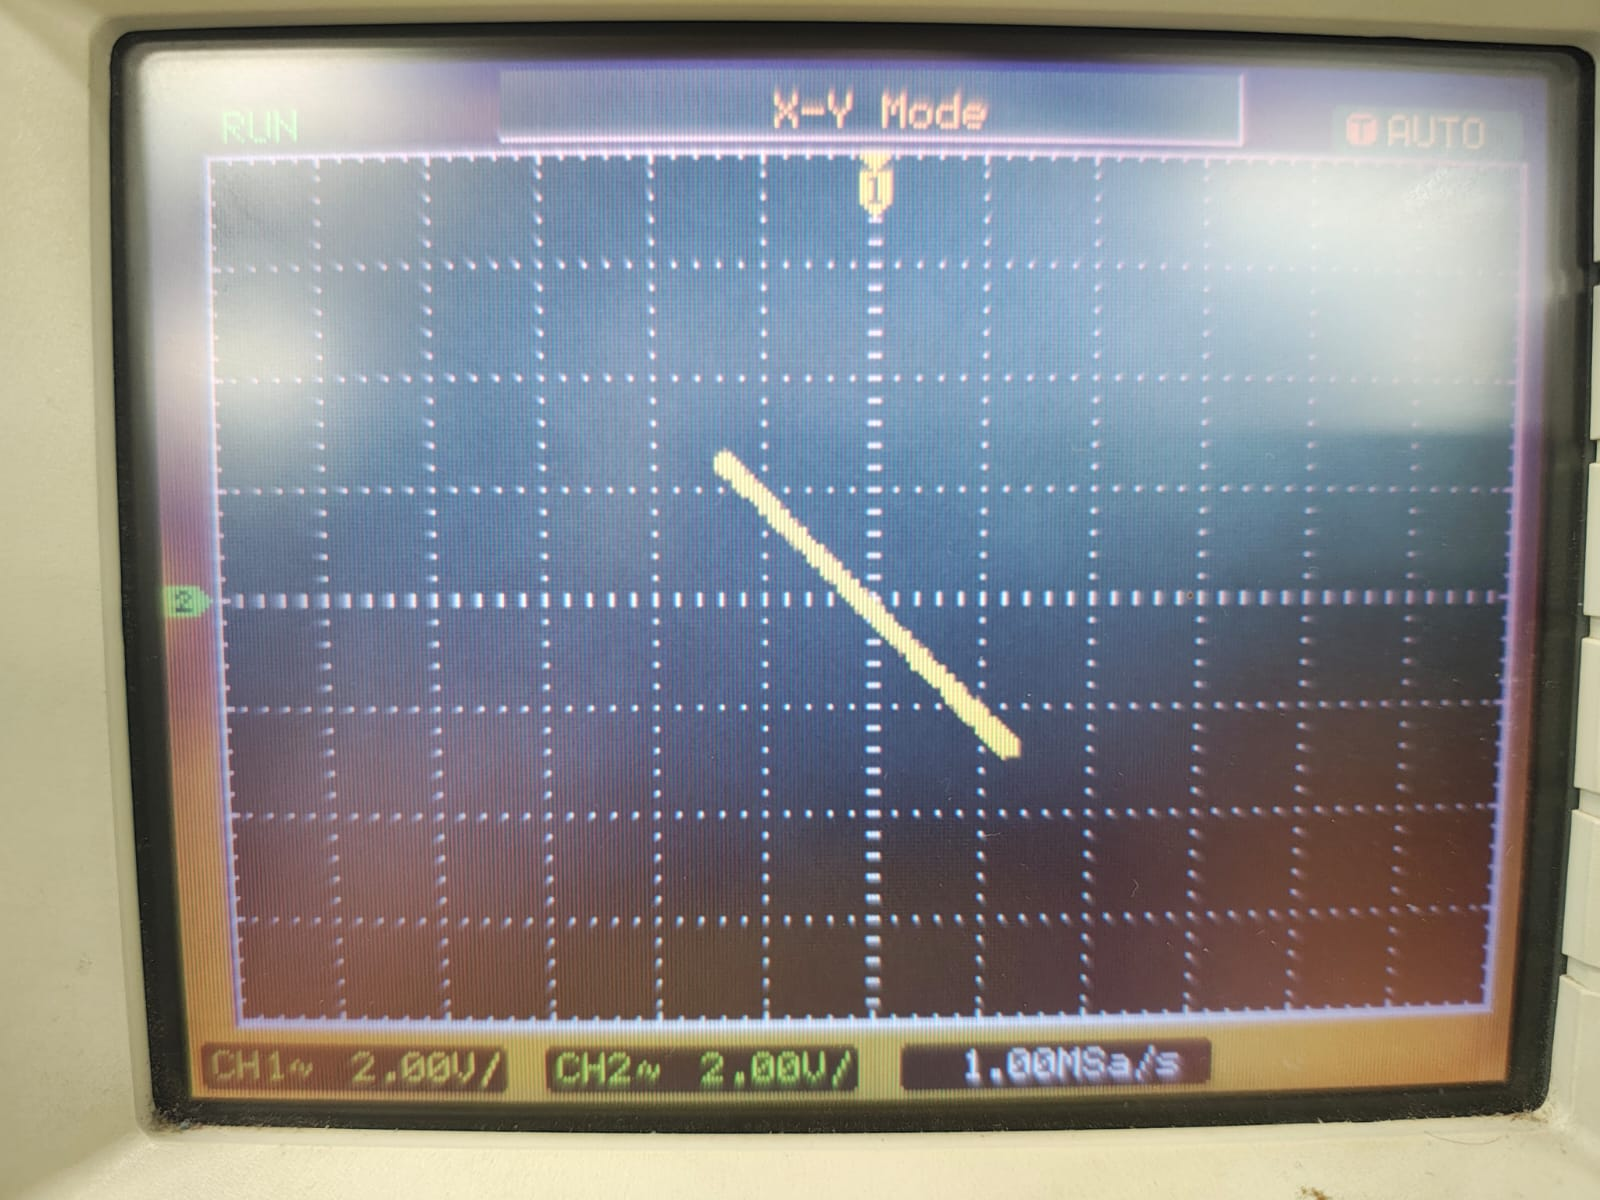
\includegraphics[width=\linewidth]{Graphs/Graph4.jpeg}
        \caption{Obtained}
    \end{minipage}
    \hfill
    \begin{minipage}{0.45\textwidth}
        \centering
        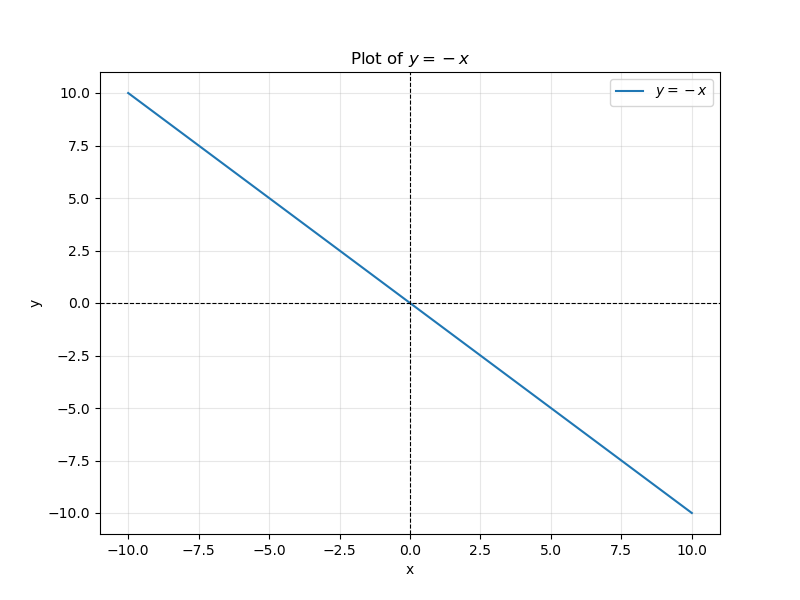
\includegraphics[width=\linewidth]{Python plots/lab6.png} 
        \caption{Generated}
    \end{minipage}
\end{figure}\\
\newpage
\section{Impulse}
\begin{itemize}
\item In addition to generating Lissajous figures, the setup can effectively capture rapidly changing signals, such as impulses, commonly referred to as "on-off" phenomena.
\item This capability allows for precise analysis of transient events within a system.
\item Notably, only a single-channel connection is required to record these signals, making the setup both efficient and simple.
\item An example of such a recorded signal is presented below.
\item This approach is particularly useful in scenarios where high-speed signal detection is critical, such as in communication systems, control circuits, or transient analysis in electronic devices.
\end{itemize}
\begin{figure}[htbp]
    \centering
    \begin{minipage}{0.45\textwidth}
        \centering
        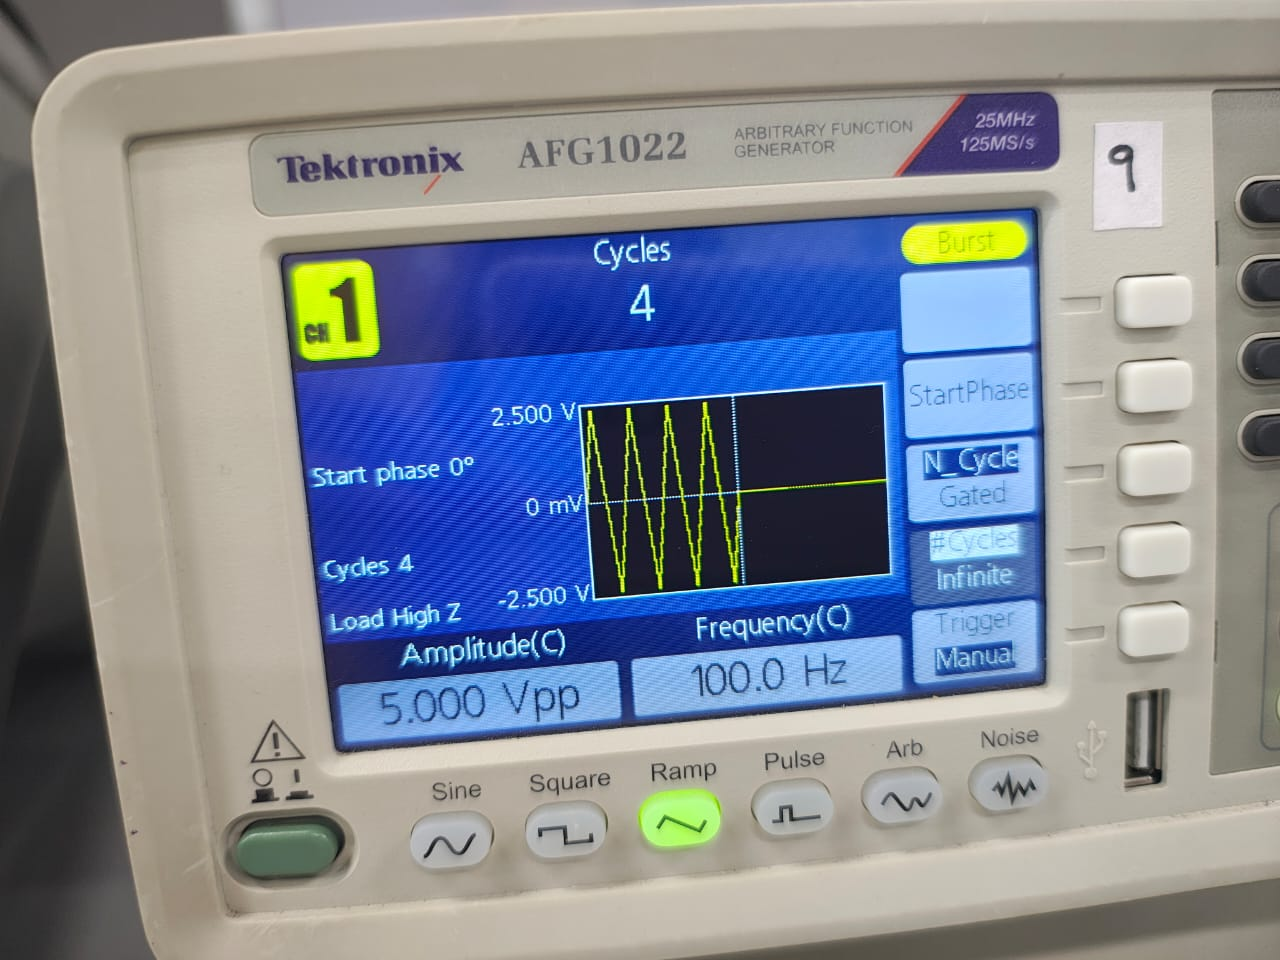
\includegraphics[width=\linewidth]{Tables/Impulse.jpeg}
        \caption{}
    \end{minipage}
    \hfill
    \begin{minipage}{0.45\textwidth}
        \centering
        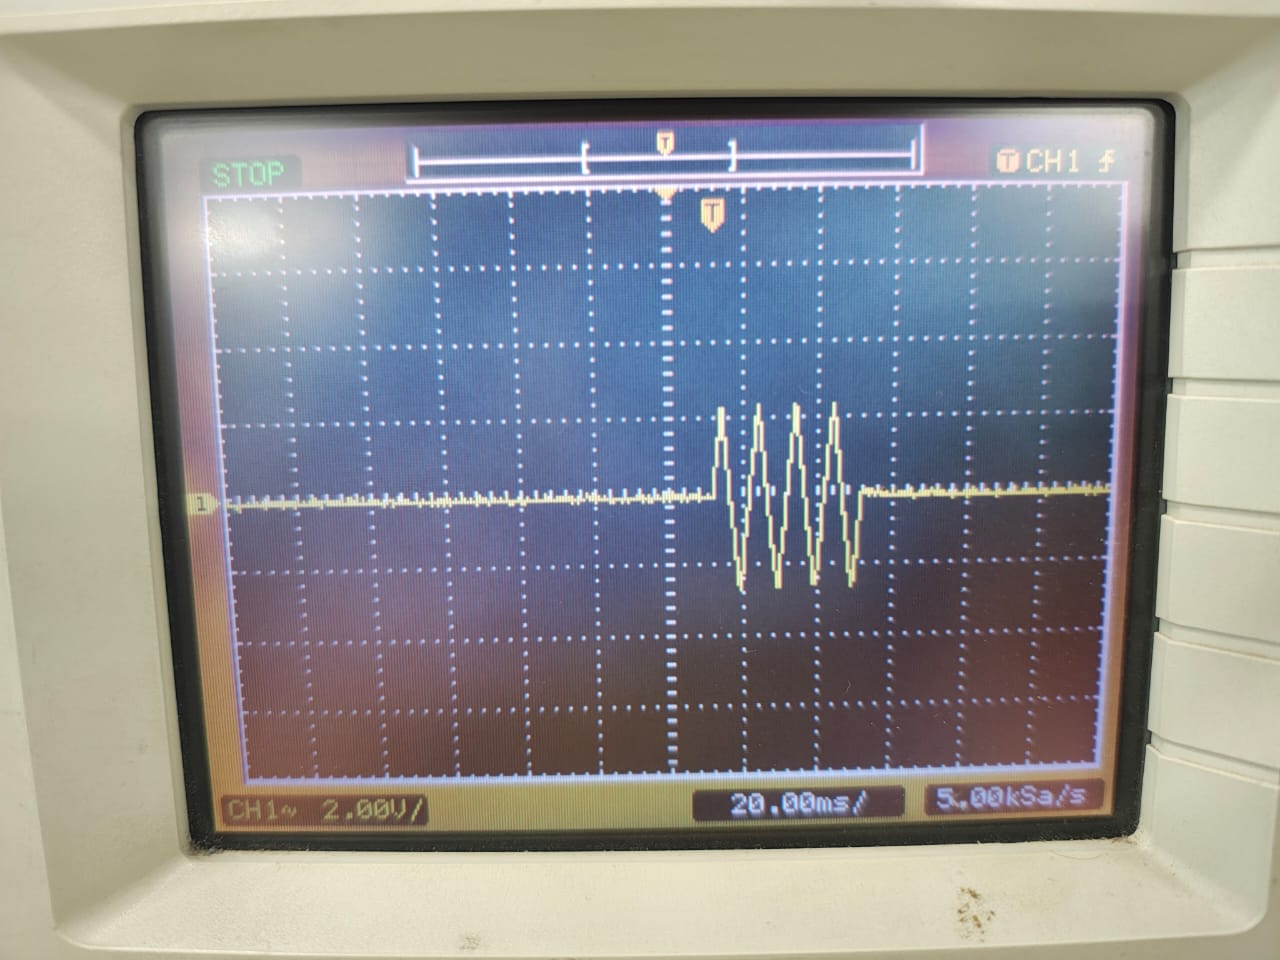
\includegraphics[width=\linewidth]{Graphs/Impulse.jpeg} 
        \caption{}
    \end{minipage}
\end{figure}
\textbf{Precautions}\\
When working with the oscilloscope and inputting signals, certain precautions must be followed to ensure accurate results and safety:
\begin{itemize}
    \item Ensure the phases of the input signals are correct, and verify that the oscilloscope is not imposing its own phase difference on the signals, as this could lead to incorrect measurements.
    \item Check that all connections are secure and not loose, as loose connections can introduce unwanted noise into the signals, potentially distorting the Lissajous figures.
    \item Always turn off the oscilloscope and related equipment before making or modifying connections to avoid the risk of electrical shocks or damage to the device.
\end{itemize}
\end{document}
